\documentclass[12pt, twoside]{article}
\usepackage[letterpaper, margin=1in, headsep=0.5in]{geometry}
\usepackage[english]{babel}
\usepackage[utf8]{inputenc}
\usepackage{amsmath}
\usepackage{amsfonts}
\usepackage{amssymb}
\usepackage{tikz}
\usepackage{yhmath}
%\usetikzlibrary{quotes, angles}

\usepackage{graphicx}
\usepackage{enumitem}
\usepackage{multicol}

\usepackage{fancyhdr}
\pagestyle{fancy}
\fancyhf{}
\renewcommand{\headrulewidth}{0pt} % disable the underline of the header

\fancyhead[RE]{\thepage}
\fancyhead[RO]{\thepage \\ Name: \hspace{3cm}}
\fancyhead[L]{BECA / Dr. Huson / 10th Grade Geometry\\* 6 February 2020}

\begin{document}
\subsubsection*{8.8 Exam: Area, volume, solids, circles review}
 \begin{enumerate}

  \item Use the formulas for the area and circumference of circles:
  \[A=\pi r^2\]
  \[C=\pi D = 2\pi r\]
  
  \item Given the circle centered at $O$ with radius $r=3$. Leave an exact answer, in terms of $\pi$ if necessary.
  \begin{multicols}{2}
    \begin{enumerate}
      \item Find the circumference of circle $O$. %\vspace{1cm}
      \item Find the area of the circle.\vspace{2cm}
    \end{enumerate}
    %\columnbreak
    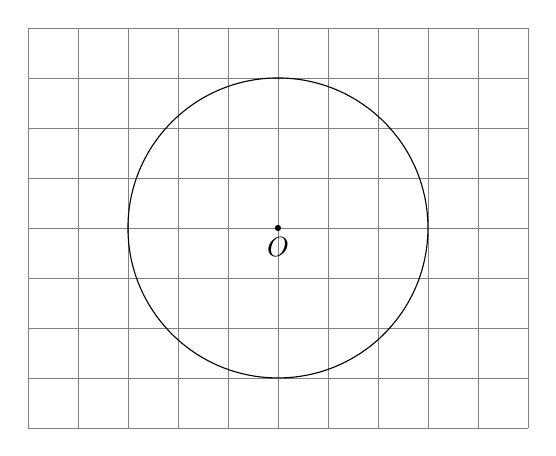
\begin{tikzpicture}[scale=.635]
      \draw [help lines] (-5,-4) grid (5,4);
      %\draw [thick, ->] (-2.2,0) -- (10.4,0) node [below right] {$x$};
      %\draw [thick, ->] (0,-2.2)--(0,10.4) node [left] {$y$};
      \draw (0,0) circle [radius=3] node[below]{$O$};
      \draw [fill] (0,0) circle [radius=0.05];
    \end{tikzpicture}
  \end{multicols}

  \item Find the radius of a circle having an area of $25 \pi$. \vspace{2cm}
  
  \item Find the area of the shape shown below composed of a rectangle and circular cap. Leave your answer as an exact value in terms of $\pi$.
    \begin{flushright}
    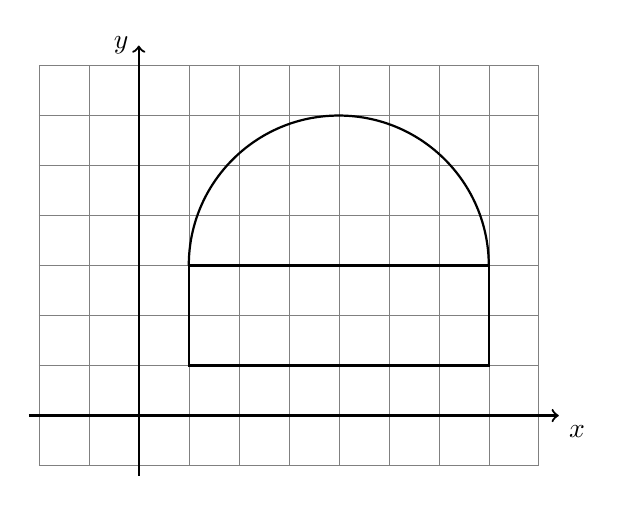
\begin{tikzpicture}[scale=.635]
      \draw [help lines] (-2,-1) grid (8,7);
      \draw [thick, ->] (-2.2,0) -- (8.4,0) node [below right] {$x$};
      \draw [thick, ->] (0,-1.2)--(0,7.4) node [left] {$y$};
      \draw [thick] (1,1)--(7,1)--(7,3)--(1,3)--cycle;
      %\draw [thick] (3,4) arc (90:270:1);
      \draw [thick] (7,3) arc (0:180:3);
    \end{tikzpicture}
  \end{flushright}\vspace{1cm}

\newpage
\item A pentagon is inscribed in circle $O$, as shown below. The circle has radius $r=9$.
    \begin{multicols}{2}
    \raggedcolumns
    \begin{enumerate}
      \item Find the area of the sector $AOB$. \vspace{3cm}
      \item Find the perimeter of the sector $AOB$. %\vspace{1.5cm}
    \end{enumerate}
      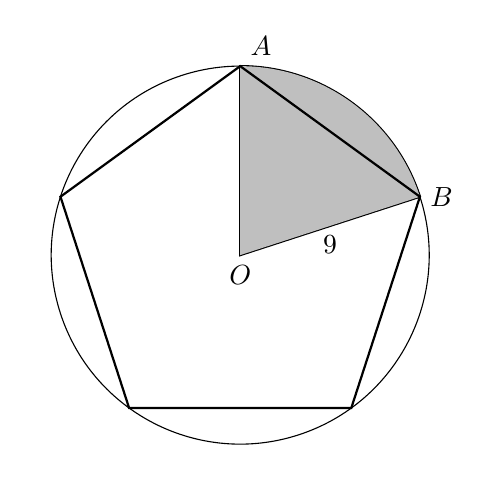
\begin{tikzpicture}[scale=0.8, rotate=18]
        \draw (0,0) circle[radius=3];
        \draw [thick]
        (0:3) node[right] {$B$}--
        (0,0) node[below] {$O$}--
        (72:3) node[above right] {$A$} arc (72:0:3);
        \fill [lightgray]
        (0,0)--(0:3) arc (0:72:3)--(0,0);
        \draw (1.5,0) node[below] {$9$};
        \draw [thick] (0:3)--(72:3)--(2*72:3)--(3*72:3)--
        (4*72:3)--cycle;
      \end{tikzpicture}
    \end{multicols}  \vspace{1cm}

    \item Given the circle with center $P$ with central angle $\angle APB$ and inscribed angle $\angle AQB$. Using a protractor, measure each angle.
  \begin{multicols}{2}
    \raggedcolumns
    \begin{enumerate}
      \item $m\angle APB=$ \vspace{0.7cm}
      \item $m\angle AQB=$ \vspace{0.7cm}
      \item What do you think is the ratio of the central angle to the inscribed angle?
    \end{enumerate}
      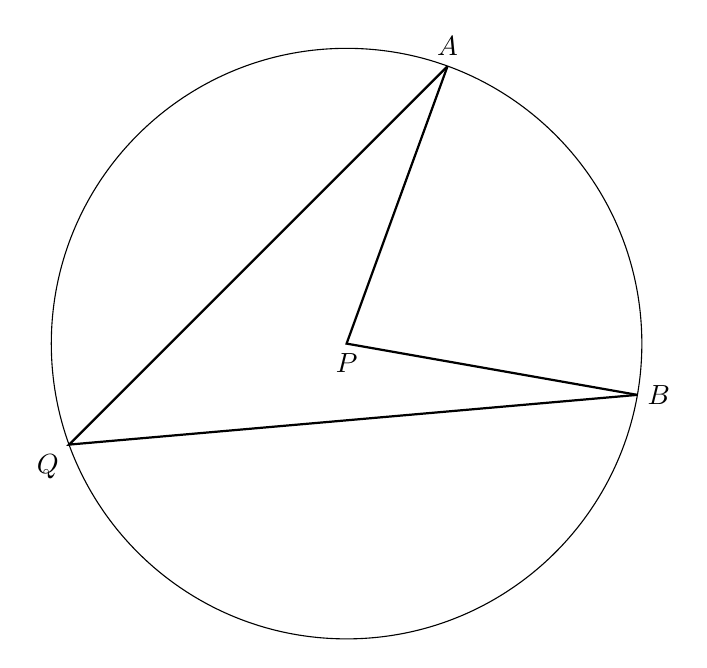
\begin{tikzpicture}[scale=.75]
        \draw (0,0) circle[radius=5];
        \draw [thick]
        (-10:5) node[right] {$B$}--
        (0,0) node[below] {$P$}--
        (70:5) node[above] {$A$};
        \draw [thick] (-10:5)--(200:5) node[below left] {$Q$}--(70:5);
        %\draw (60:5) node[right]{$130^\circ$};
      \end{tikzpicture}
  \end{multicols}

  \item Given $R(-3,1)$ and $S(5,7)$, find the length of $\overline{RS}$. Note: $l=\sqrt{(x_2-x_1)^2+(y_2-y_1)^2}$. %\vspace{4cm}
  
\newpage
  \item Perform each calculation, writing down the full calculator display and then rounding to the \emph{nearest hundredth}.
  \begin{multicols}{2}
  \begin{enumerate}
    \item $V=\frac{1}{3} \pi (2.4)^2(5.1)$
    \item $P=3.6 + \frac{1}{2} \pi (3.6)$  
  \end{enumerate}
  \end{multicols}\vspace{2cm}

  \item Solve each equation for the appropriate variable. Do not round. Simplify radicals.
  \begin{multicols}{2}
  \begin{enumerate}[itemsep=2cm]
    \item $A=\pi r^2=27\pi$
    \item $V=\frac{1}{3}(6.0)^2h=153$  
  \end{enumerate}
  \end{multicols}\vspace{5cm}

  \subsubsection*{Model the situation with an equation. Use the formula sheet. You must start with a labeling variable. \hfill Do NOT solve!}

  \item A large concrete post in the shape of a cylinder has a volume of 250 cubic feet. Its height is 12 feet. Find the radius of the base of the post. \vspace{2cm}

  \item A spherical cork fishing net float has a volume of 4000 cubic centimeters. Find its radius. \vspace{2cm}

  \item The volume of a cone having a \textbf{diameter} of 10 inches is 200 cubic inches. Find the cone's height. \vspace{2cm}

  \newpage
  \subsubsection*{Applying density ratios}
  \item A tank of gasoline holds 15 gallons. Find the cost to completely fill the tank if gasoline costs \$3.15 per gallon. \vspace{3cm}
  \item A stick of butter has a volume of 90 cubic centimeters. If the density of butter is 0.9 grams per cubic centimeter, find the weight of a stick of butter. \vspace{3cm}
  \item A large glass marble has a diameter of 3 cm. The density of glass is 2.70 $\mathrm{g/cm}^3$. Find the weight of the marble. \vspace{3cm}

  \item A bar of solid gold is in the shape of a rectangular prism having a length of 12 cm, width of 2 cm, and thickness of 2 cm. The density of gold is 19.3 grams per cubic cm, and its approximate market value is \$50 per gram.
  \begin{enumerate}
    \item Find the weight of the bar of gold.  \vspace{3cm}
    \item Find its value in dollars.
  \end{enumerate}

\newpage
  \item Circle the number of the correct choice. \\
    \includegraphics[scale=0.42]{triangle-rotation.png}

\item %January 2018
  Circle $P$ is centered at the origin. In the diagram below, half of circle $P$ is graphed.
    \begin{center}
      \begin{tikzpicture}[scale=0.6]
        %\draw [help lines] (-4,-4) grid (4,4);
        \draw [thick, <->] (-4,0) -- (4,0) node [below right] {$x$};
        \draw [thick, <->] (0,-3)--(0,3) node [left] {$y$};
        %\draw (0,0) circle [radius=2];
        \draw [thick] (0,2) arc (90:270:2);
        \node at (0,0) [above right]{$P$};
      \end{tikzpicture}
      \end{center}
    Which three-dimensional figure is generated when the semi-circle is continuously rotated about the $y$-axis?
    \begin{multicols}{2}
      \begin{enumerate}
      \item cone
      \item sphere
      \item cylinder
      \item hemisphere
      \end{enumerate}
    \end{multicols}

  \item %January 2018
  A right hexagonal prism is shown below. A two-dimensional cross section that is parallel to the base is taken from the prism.
    \begin{center}
    \includegraphics[scale=0.4]{hex-prism_JA2018.png}
    \end{center}
   Which figure describes the two-dimensional cross section?
    \begin{multicols}{2}
      \begin{enumerate}
        \item rectangle
        \item trapezoid
        \item pentagon
        \item hexagon
      \end{enumerate}
    \end{multicols}

\newpage
\subsubsection*{Vocabulary: Circles (fill in the blank with the correct term)}

  \item \textbf{Internal line segments:} Circle with center at point $P$, as shown.
    \begin{multicols}{2}
      \begin{enumerate}
        %\item  $\overline{AB}$ \quad \rule{3cm}{0.15mm} %Diameter
        \item  $\overline{CP}$ \quad \rule{3cm}{0.15mm} %Radius
        \item  $\overline{DE}$ \quad \rule{3cm}{0.15mm} %Chord
        \item $\angle APC$ \quad \rule{3cm}{0.15mm} %Central angle 
        \item  $\wideparen{AC}$ \quad \rule{3cm}{0.15mm} %(with measure $m\wideparen{AC} = 72^\circ$)Arc
      \end{enumerate}
    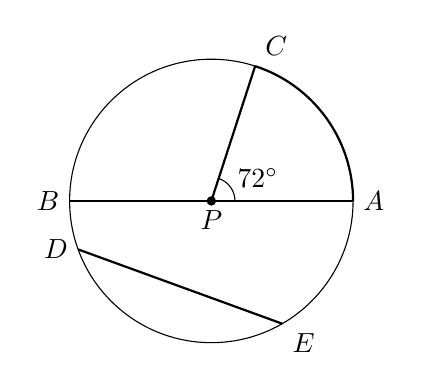
\begin{tikzpicture}[scale=0.6]
      \draw (0,0) circle[radius=3];
      \draw [thick] (3,0) arc (0:72:3);
      \draw [thick] (0:3) node[right] {$A$}--(180:3) node[left] {$B$};
      \draw [thick] (0,0)--(72:3) node[above right] {$C$};
      \draw [thick] (200:3) node[left] {$D$}--(300:3) node[below right] {$E$};
      \fill (0,0) circle[radius=0.1] node[below]{$P$};
      \draw (0.5,0) arc (0:72:0.5) node[right]{$\ 72^\circ$};
      %\draw (35:5) node[right] {$\wideparen{AC}$};
      %\draw (290:5) node[below] {$D$};
    \end{tikzpicture}
  \end{multicols}

  \item \textbf{External lines:} Circle with center at point $O$, at right.
    \begin{multicols}{2}
      \begin{enumerate}
        \item  $\overline{FGH}$ \quad \rule{3cm}{0.15mm} %Secant
        \item  $\overline{OJ}$ \quad \rule{3cm}{0.15mm} %Radius
        \item  $\overline{FJK}$ \quad \rule{3cm}{0.15mm} %Tangent
        \item $J$ \quad \rule{3cm}{0.15mm} %Point of tangency 
        %\item Note: $\overline{OJ} \perp \overline{FJK}$
      \end{enumerate}
    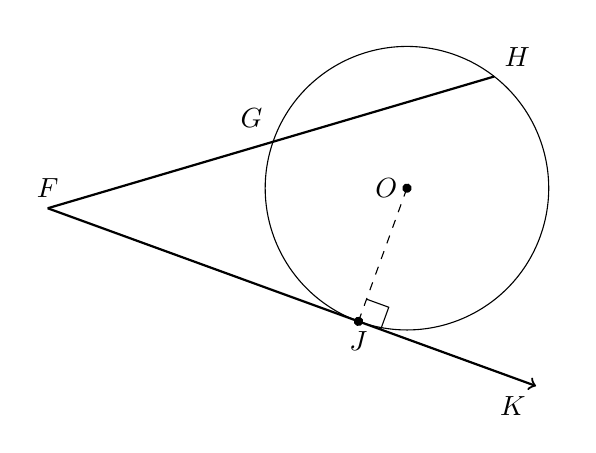
\begin{tikzpicture}[scale=0.6, rotate=-20]
      \draw (0,0) circle[radius=3];
      \draw [thick, ->] (-7,-3) node[above] {$F$}--(4,-3) node[below left] {$K$};
      \draw [thick] (-7,-3)--(72:3) node[above right] {$H$};
      \draw [dashed] (0,-3) node[below] {$J$}--(0,0);
      \fill (0,0) circle[radius=0.1] node[left]{$O$};
      \fill (0,-3) circle[radius=0.1];
      \draw (0,-3) ++(0.5,0)-- ++(0,0.5)--++(-0.5,0);
      \draw (170:3.8) node[below] {$G$};
    \end{tikzpicture}
  \end{multicols}
    
  \item \textbf{Areas:} Circle with center at point $Q$.
    \begin{multicols}{2}
      \begin{enumerate}
        \item  $\overline{RS}$ \quad \rule{3cm}{0.15mm} %Diameter
        \item  $RST$ \quad \rule{3cm}{0.15mm} %Semi-circle
        \item  $QUV$ \quad \rule{3cm}{0.15mm} %Sector
      \end{enumerate}
    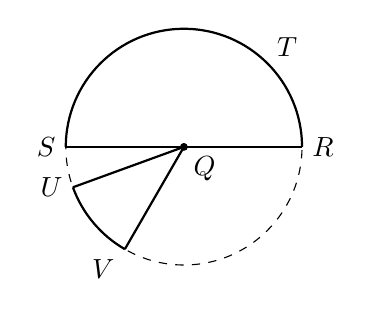
\begin{tikzpicture}[scale=0.5]
      \draw [dashed](0,0) circle[radius=3];
      \draw [thick] (0,0) ++(3,0) arc (0:180:3);
      \draw [thick] (200:3) arc (200:240:3);
      \draw [thick] (0:3) node[right] {$R$}--(180:3) node[left] {$S$};
      \draw [thick] (0,0)--(200:3) node[left] {$U$};
      \draw [thick] (0,0)--(240:3) node[below left] {$V$};
      \fill (0,0) circle[radius=0.1] node[below right]{$Q$};
      \draw (50:3.3) node[right] {$T$};
    \end{tikzpicture}
  \end{multicols}

  \begin{multicols}{2}
  \item \textbf{Polygons and angles in circles:} %Circle with triangle inscribed.
      \begin{enumerate}
        \item  $\triangle XYZ$ \vspace{0.5cm} \quad \rule{3cm}{0.15mm} %Inscribed
        %\item  $\angle XYZ$ \quad \rule{3cm}{0.15mm} %Inscribed
      \end{enumerate} \hspace{1cm}
    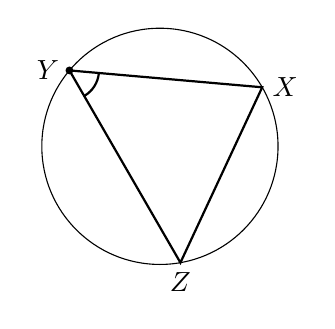
\begin{tikzpicture}[scale=0.5]
      \draw (0,0) circle[radius=3];
      \draw [thick] (140:3) ++(-60:0.75) arc (-60:-5:0.75);
      \draw [thick] (30:3) node[right] {$X$}--(140:3) node[left] {$Y$}
      --(280:3)node[below] {$Z$}--cycle;
      %\draw [thick] (0,0)--(200:3) node[left] {$U$};
      %\draw [thick] (0,0)--(240:3) node[below left] {$V$};
      \fill (140:3) circle[radius=0.1];
      %\draw (50:3.3) node[right] {$T$};
    \end{tikzpicture}
  \end{multicols}

\newpage
\item The diagram shows the sector $AOB$ in circle $O$. The circle has radius $r=7$.
    \begin{multicols}{2}
    \raggedcolumns
    \begin{enumerate}
      \item Find the area of the entire circle $O$ in terms of $\pi$. \vspace{2cm}
      \item The sector $AOB$ has an area of $16 \frac{1}{3}\pi$. What fraction of the entire circle is it? \vspace{1.5cm}
      \item Find the measure of central angle $\theta$.
    \end{enumerate}
      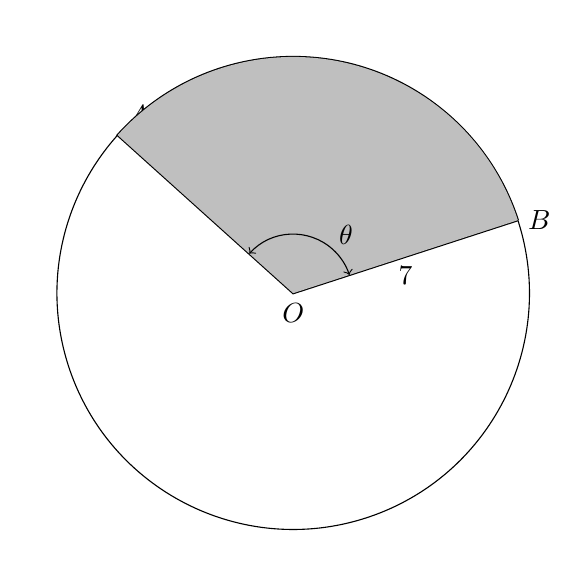
\begin{tikzpicture}[scale=1, rotate=18]
        \draw (0,0) circle[radius=3];
        \draw [thick]
        (0:3) node[right] {$B$}--
        (0,0) node[below] {$O$}--
        (120:3) node[above right] {$A$} arc (120:0:3);
        \fill [lightgray]
        (0,0)--(0:3) arc (0:120:3)--(0,0);
        \draw [<->] (120:0.75) arc (120:0:0.75);
        \node at (30:1){$\theta$};
        \draw (1.5,0) node[below] {$7$};
        %\draw [thick] (0:3)--(72:3)--(2*72:3)--(3*72:3)--(4*72:3)--cycle;
      \end{tikzpicture}
    \end{multicols}  \vspace{2cm}

\item Given quadrilateral $CDEH$ with $C(-8,2)$, $D(-3,4)$, $E(-1,-1)$, and $H(-6,-3)$. Find its perimeter.
  \begin{flushright}
    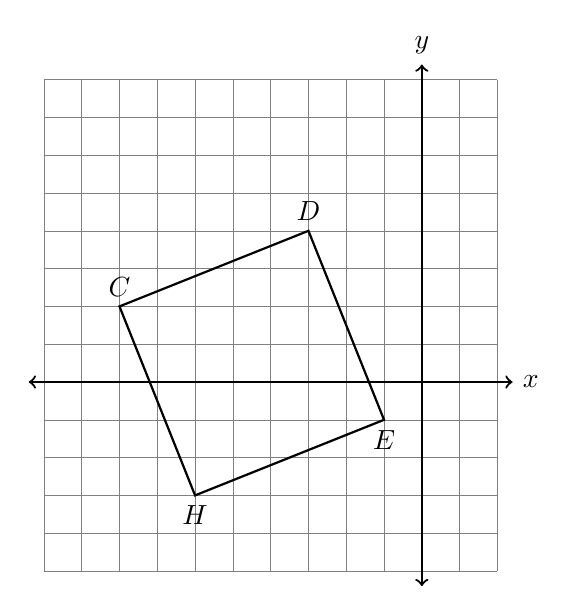
\begin{tikzpicture}[scale=.48]
      \draw [help lines] (-10,-5) grid (2,8);
      \draw [thick, <->] (-10.4,0) -- (2.4,0) node [right] {$x$};
      \draw [thick, <->] (0,-5.4)--(0,8.4) node [above] {$y$};  
      \draw [thick]
        (-8,2) node[above] {$C$}--
        (-3,4) node[above] {$D$}--
        (-1,-1) node[below] {$E$}--
        (-6,-3) node[below] {$H$}--cycle;
      %\draw [thick](-5,5)--(-1,-1);
      %\draw [thick](2,5)--(-8,-1);
      %\draw [fill] (-3,2) circle [radius=0.1]node[left]{$P$};
  \end{tikzpicture}
  \end{flushright}
  Justify that $CDEH$ is a rhombus.

\newpage
  \item A rectangle has two triangular cutouts as shown with lengths marked. Find the area of the figure. (the figure is not drawn to scale)
  \begin{flushleft}
  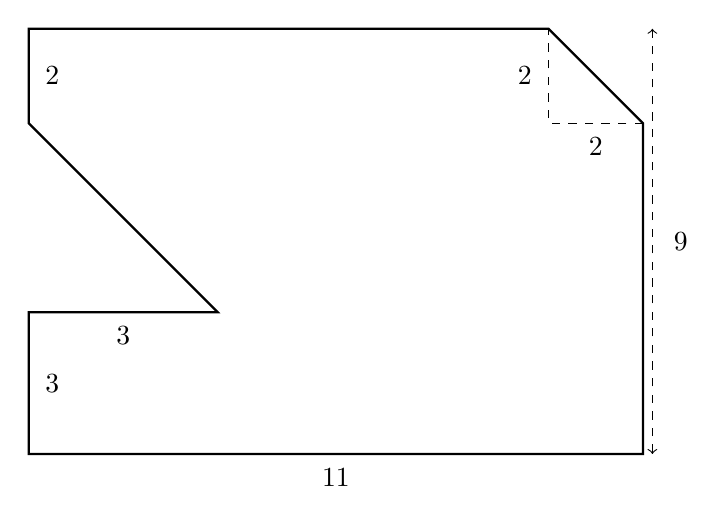
\begin{tikzpicture}[scale=0.6]
    \draw [-, thick] (0,0)--(13,0)--(13,7)--(11,9)--
    (0,9)--(0,7)--(4,3)--(0,3)--cycle;
    \draw [dashed] (13,7)--(11,7)--(11,9);
    \draw [<->, dashed] (13.2,0)--(13.2,9);
    %\draw [fill] (0,0) circle [radius=0.05] node[left]{$A$};
    %\draw [fill] (7,0) circle [radius=0.05] node[right]{$B$};
    %\draw [fill] (7,2) circle [radius=0.05] node[right]{$C$};
    %\draw [fill] (0,2) circle [radius=0.05] node[left]{$D$};
    \node at (0.5, 8){2};
    \node at (0.5, 1.5){3};
    \node at (2, 2.5){3};
    \node at (10.5, 8){2};
    \node at (12, 6.5){2};
    \node at (6.5, -0.5){11};
    \node at (13.8, 4.5){9};
    %\node at (13.5, 8){2};
  \end{tikzpicture}
  \end{flushleft} \vspace{3cm}

  \item A trapezoid has a height of 11.5 and one perpendicular side, as shown below. One base is six longer than the shorter base. \\[0.25cm]
    If the trapezoid has an area of 276, find the lengths of the bases.
    \begin{flushright} 
    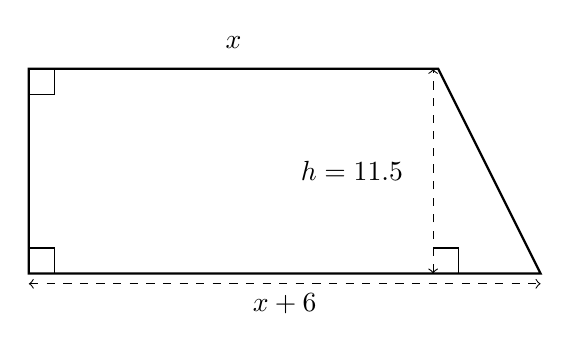
\begin{tikzpicture}[scale=1.3]
      \draw [thick]
      (3,0)--(3,2)--(7,2)--(8,0)--cycle;
      \draw [dashed,<->] (6.95,0)--(6.95,2);
      %\draw [dashed,<->] (0,2.1)--(7,2.1);
      %\draw [->] (45:0.5)--(45:0.9142);
      %\draw [->] (45:2.3)--(45:1.9142);
      \draw (3,0)++(0,0.25)--++(0.25,0)--+(0,-0.25);
      \draw (3,2)++(0,-0.25)--++(0.25,0)--+(0,0.25);
      \draw (6.95,0)++(0,0.25)--++(0.25,0)--+(0,-0.25);
      \draw [dashed,<->] (3,-0.1)--(8,-0.1);
      \node at (5.5,-0.1)[below]{$x+6$};
      \node at (6.75,1)[left]{$h=11.5$};
      \node at (5,2.1)[above]{$x$};
    \end{tikzpicture}
    \end{flushright} 
    \vspace{4cm}

\end{enumerate}
\end{document}
